\documentclass[a4paper, 11pt]{article}
\usepackage{comment} % enables the use of multi-line comments (\ifx \fi) 
\usepackage{fullpage} % changes the margin
\usepackage[german]{babel}
\usepackage[utf8]{inputenc}
\usepackage{graphicx}
\usepackage{multicol}
\usepackage{float}
\usepackage{fancyhdr}
\usepackage{enumitem}
\pagestyle{fancy} 
\usepackage{pdfpages}
%\usepackage[head=128pt]{geometry}
\title{Sitzungs-protokoll}
\author{Christian Kirfel}
\usepackage[margin=1in]{geometry}
\setlength{\footskip}{0.1pt}
\setlength{\headheight}{80pt}
\setlength{\topmargin}{0pt}
\setlength\parindent{0pt}
\fancypagestyle{style1}{
\rhead{
\includegraphics[width=4cm]{logo_catena}}
\cfoot{
\makebox{}\\
\makebox{}\\
\hspace{15cm}
\makebox[0.1\linewidth]{\rule{0.1\linewidth}{0.1pt}} \hspace{1cm} \makebox[0.1\linewidth]{\rule{0.1\linewidth}{0.1pt}} \hspace{1cm} \makebox[0.1\linewidth]{\rule{0.1\linewidth}{0.1pt}} \hspace{1cm} \makebox[0.1\linewidth]{\rule{0.1\linewidth}{0.1pt}} \hspace{1cm}\\}
}

\newcommand\signature[2]{% Name; Department
\noindent\begin{minipage}{5cm}
    \noindent\vspace{3cm}\par
    \noindent\rule{5cm}{1pt}\par
    \noindent\textbf{#1}\par
    \noindent#2%
\end{minipage}}



\begin{document}
\pagestyle{style1}

\textbf{Datum: 19.09.2020} % inserir data aqui
\textbf{Sitzungszeit: 15:00 - 15:50}
\textbf{Ort: Remote, Zoom} % Definir local da reunião 

\textbf{Teilnehmer:} %
\begin{description}
\item Martin Reinicke, Vorsitzender
\item Dr.~Michael Schumacher, stellv. Vorsitzender
\item Volker Nießen, Geschäftsführer
\item Friedhelm Schmitt, Kassenprüfer
\item Christian Kirfel, Schriftführer
\item Jörg Zwitters, Verbindungslehrer
\item Leonhard Paulig, Kassenprüfer
\item Dominik Hoven, Beisitzer
\item Yannick Hansen, Beisitzer
\item Max Frauenrath, Beisitzer
\item Philip Lanio, Beisitzer
\item Thomas Frauenkron, Schulleiter
\item Dirk Udo Fricke, Mitglied
\item Günter M. Lutsch, Mitglied
\end{description}

\makebox[\linewidth]{\rule{\linewidth}{0.4pt}}\\
\textbf{Programmpunkte:} 
\begin{enumerate}
\item Begrüßung
\item Feststellung der Beschlussfähigkeit
\item Genehmigung des Protokolls der MV September 2019
\item Bericht des Vorstandes
\item Bericht des Schatzmeisters
\item Bericht des Kassenprüfers
\item Entlastung des Vorstandes
\item Wahl des Vorsitzenden, Wahl des Schatzmeisters, Wahl eines Kassenprüfers
\item Persönliche Anträge
\item Verschiedenes
\end{enumerate}
\makebox[\linewidth]{\rule{\linewidth}{0.4pt}}\\

\newpage

\section*{Begrüßung}

Die Verwaltung der Mitglieder wird von Volker übernommen

Zur Nutzung von Meinverein ist ein Buhl Account notwendig.
Dies sollte kommuniziert werden.
Der Vorstand testet die website.

Am besten wäre es neue Mitglieder nur noch digital anzumelden und kein Formular mehr zu nutzen.
Auf dem Schulfest könnte dies über einen QR COde oder mit einem Ipad passieren.

Das feedback zum Catena shirt ist grundsätzlich positiv. 
Beim design und möglichem Verkauf gibt es verschiedene, sehr orthogonale Meinungen.
Letztlich sind alle dafür und das design wird wenn nötig denen überlassen, die die Zeit haben, sich darum zu kümmern.

Christian geht davon aus, einen workshop im nächsten Quartal anbieten zu können.

Dominik wird neuer Ansprechpartner zur Berufsberatung. Er soll die Organisation etwaiger Orientierungstage übernehmen.

Für die SV wird ein neuer Ansprechpartner gesucht. Vorgeschlagen werden Kimberly Sarlette und Michael Schnitzler.
Letzterer war an Arbeit für die Catena interessiert. Erstere war selber in der SV.


Notizen

Es sollte kommuniyiert werden, dass wir uns freuen bald wieder ein Fest zu haben. Ein Datum soll nicht genannt werden.
Das Problem der Mitglieder ohne Email Adresse besteht weiterhin.
Man kann bei der Schule anfragen, ob es noch Bilder der Masterclass Teilchenphysik 2019 gibt. (Blog)
Die Kommunikation mit Mitgliedern wird diskutiert. Wir wollen Methoden finden Alumni und Schüler zu ermutigen in Kontakt zu treten und Hilfe anzubieten.


Michael Kratz anschrieben vorher Schnitzler
Bedarfsanalyse
Jemand muss mit der SV reden
Volker verwaltet die Mitglieder

Persönlich anschrieben
Ermutigen
Subvention

Tshirts für vorstand super

von manchen Mitgliedern haben wir keine email adresse
oder sonst keine kommunikation aber geld wir eingezogen


Die Hauptversammlung findet wegen Covid 19 digital statt.


\section*{Beschlussfähigkeit}

Die Beschlussfähigkeit wird auf Antrag des Vorsitzenden festgestellt.

\section*{Genehmigung des Protokolls der MV September 2019}

Das Protokoll wird ohne Widerspruch genehmigt.

\section*{Bericht des Vorstandes}

\subsection*{Kloster und Stiftung}

Das SSV Wochenende wurde erneut von der Catena unterstützt. Hierzu fand im September ein Besuch im Landtag Düsseldorf statt.
Eine neue Schülervertretung war für kleinere Projekte zuständig und wurde von der Catena in ihren Aufgaben unterstützt.

Die durch die Stiftung angepassten Sitzmöbel werden verwendet.

\subsection*{Schule}

Durch die Digitalisierung musste in Steinfeld kein Unterricht wegen der Pandemie ausfallen.
Thomas Frauenkron berichtet von einer neuen großen Schülervertretung, die ebenfalls erfolgreich arbeitet und in Zusammenarbeit mit Dr.~Michael Schumacher in Kontakt mit der Catena steht.
Das Verhältnis der Catena zur Schule hat sich über die letzten Jahre durch die Auflösung des Internats gewandelt und daher wird vermehrt versucht im Schulalltag frühe Assoziationen mit der Schule aufzubauen.
Hierbei versucht die Catena mehrheitlich das Feiern in der Schule zu unterstützen.

Jörg Zwitters berichtet, dass das HJK von Corona nicht unvorbereitet getroffen wurde. Durch die Digitalisierung war die Schule gut auf einen digitalen Unterricht vorbereitet. Das feedback seitens der Eltern war positiv.
Seit dem Sommer findet der Unterricht wieder in Person statt.
Die Segel-AG konnte in diesem Jahr leider nicht stattfinden. Reparaturen an der Amadeus wurden durchgeführt. Im nächsten Jahr können vorausssichtlich Segelkurse stattfinden.

Die Schule ist nun digital vollausgestattet. Das heißt, dass alle Schüler mit Ipads ausgestattet sind und mit diesen umgehen können.
In der Schule wurden Glasfaserkabel verlegt, um die Vernetzung innerhalb des Hauses zu beschleunigen.
Die Finanzierung ist durch den Digitalpakt gewährleistet.

Steinfeld bleibt eine dreizügige Schule und hatte etwa 90 gute Anmeldungen. Es mussten wenige Schüler abgelehnt werden. Dazu wurden zuvor zahlreiche Telefonate durch den Unterstufenkoordinator Burkhard Ohlerth geführt.
Hier muss auch in der Öffentlichkeitsarbeit behutsam mit den Bedürfnissen und Ängsten der Eltern und Familien im weiteren Sinne umgegangen werden.
Ein Tag der offenen Tür ist im Rahmen eines Hygienekonzepts geplant. Dabei soll der Tag der offenen Tür so gut wie möglich seinen Charme der Offenheit behalten, sofern dies im Rahmen der Hygieneregeln möglich ist.
Die Catena soll erneut vor Ort sein und fest in Führungen eingebaut werden.




\subsection*{Kloster/Kuratorium}

Das Gästehaus ist weiter gut besucht. Trotz wegfallender Seminare ist die Auslastung sehr gut.
Das Haus der Benediktineriennen wurde auch in die Gruppe der Scheitweiler Häuser aufgenommen.

Die Stiftung erhält mit Martin Reinicke einen neuen Vorsitz, nach dem Ausscheiden von Helmut Lanio.


\section*{Bericht des Schatzmeisters}

Dr.~Michael Schumacher berichtet über die Finanzen. Hierzu wurden die Folien ins Protokoll übernommen. (Abbidlugen \ref{fig:kasse1}, \ref{fig:kasse2} und \ref{fig:kasse3})

\begin{figure}
    \centering
    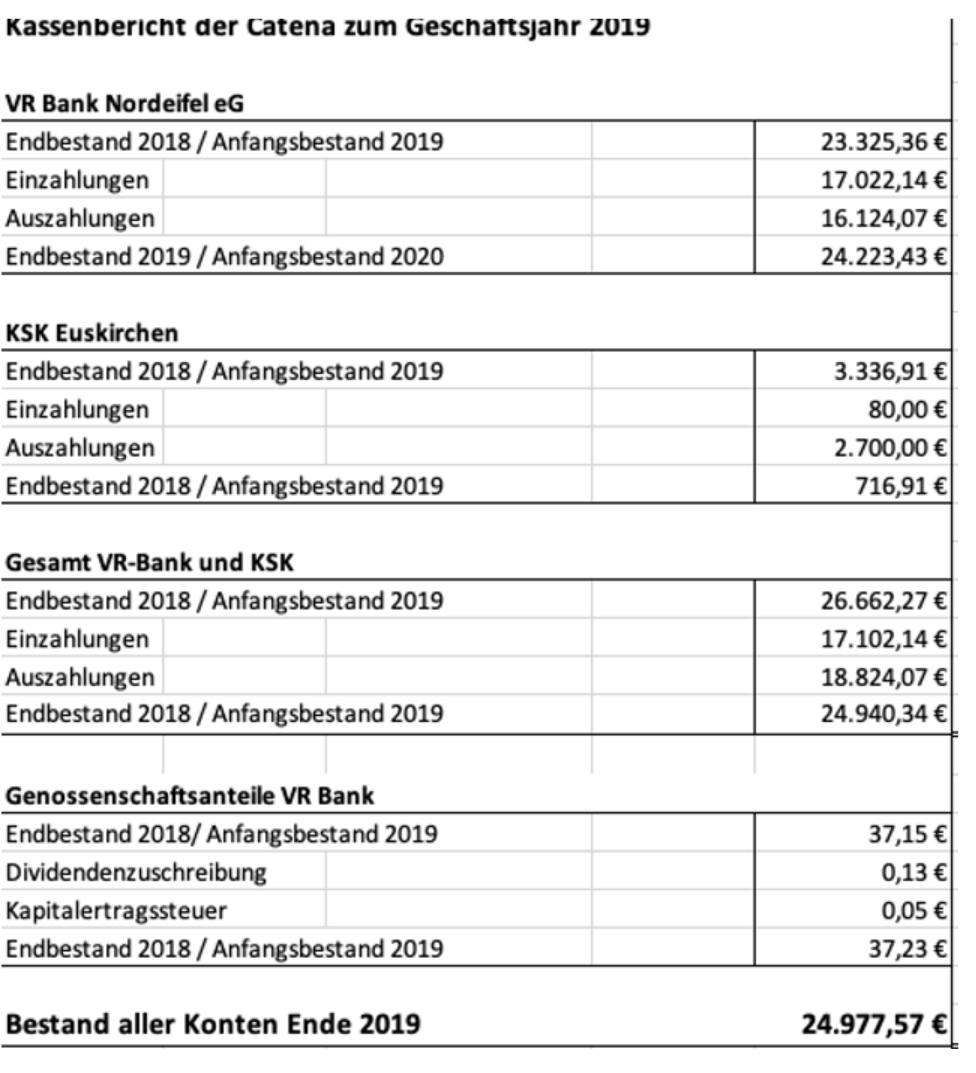
\includegraphics[width=0.8\textwidth]{kasse1.PNG}
    \caption{Bericht des Schatzmeisters, entnommen aus den Folien aus der Hauptversammlung.}
    \label{fig:kasse1}
\end{figure}

\begin{figure}
    \centering
    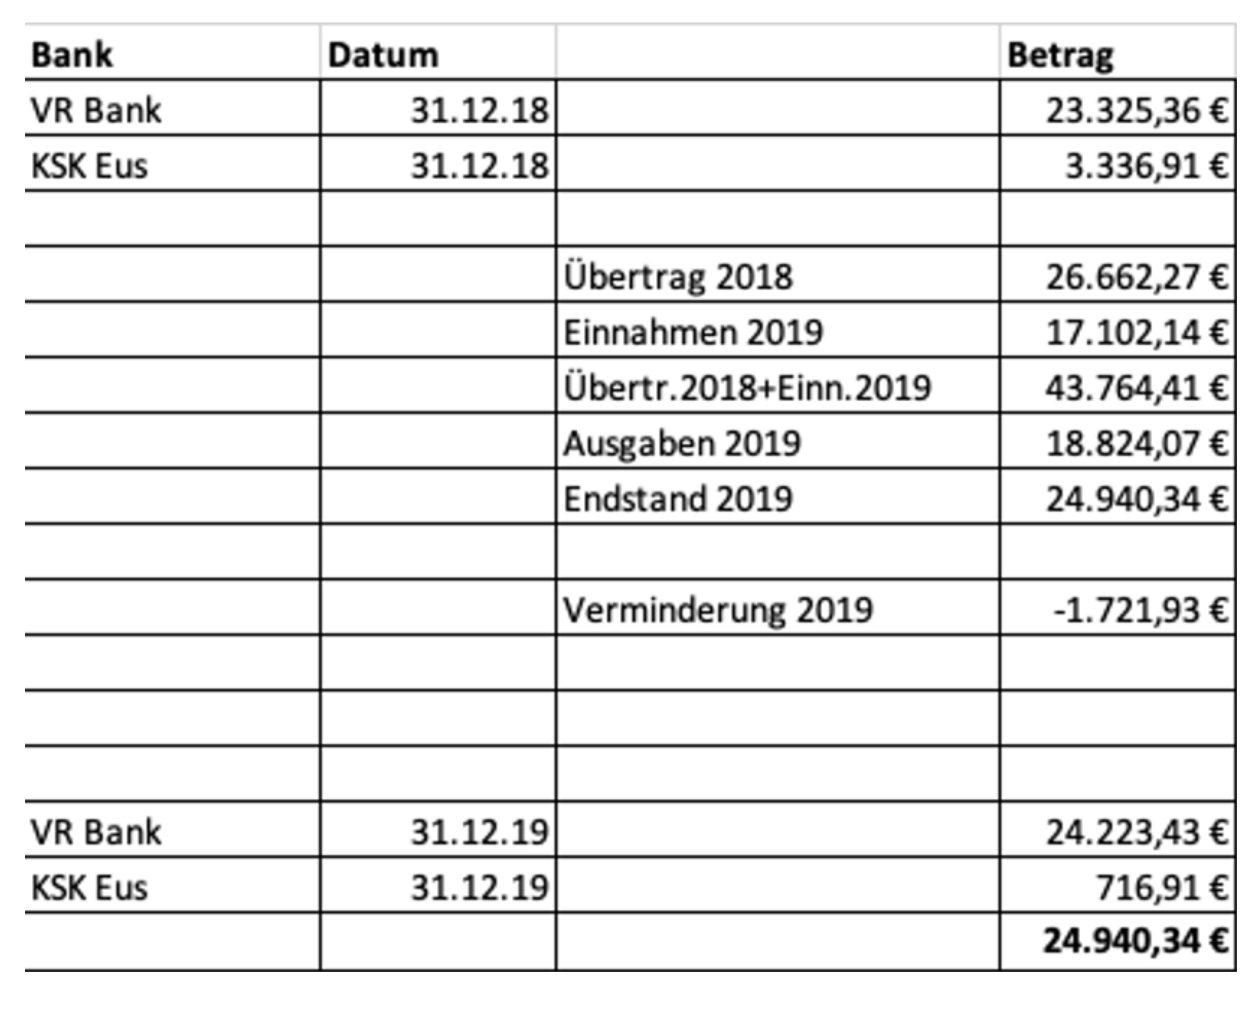
\includegraphics[width=0.8\textwidth]{kasse2.PNG}
    \caption{Bericht des Schatzmeisters, entnommen aus den Folien aus der Hauptversammlung.}
    \label{fig:kasse2}
\end{figure}

\begin{figure}
    \centering
    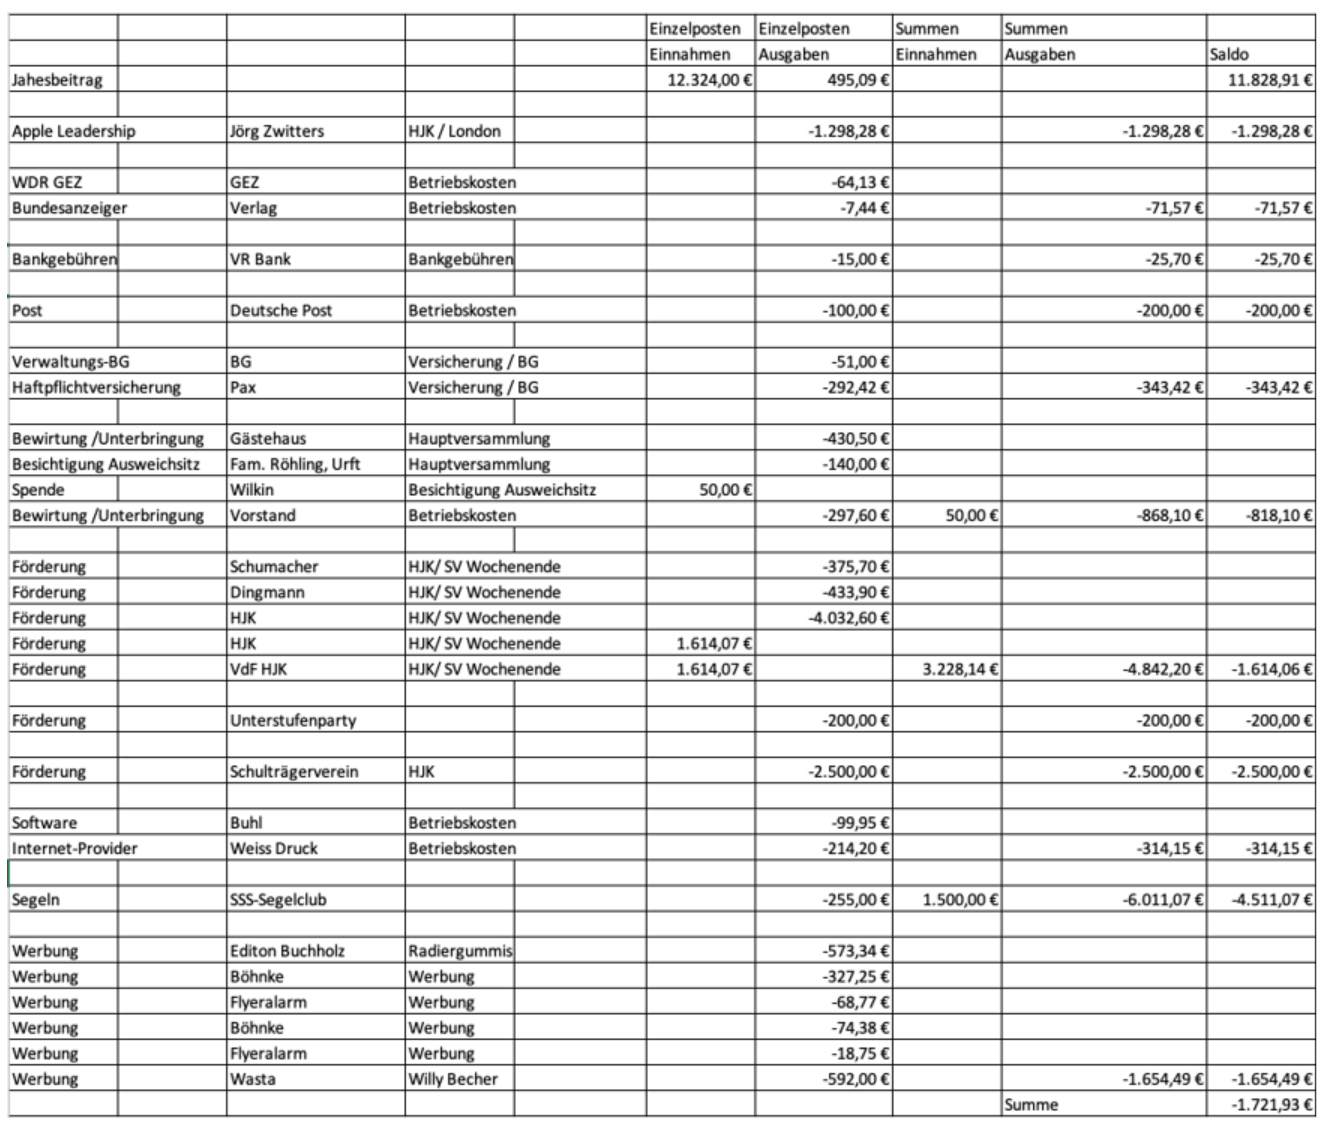
\includegraphics[width=0.8\textwidth]{kasse3.PNG}
    \caption{Bericht des Schatzmeisters, entnommen aus den Folien aus der Hauptversammlung.}
    \label{fig:kasse3}
\end{figure}


\section*{Bericht des Kassenprüfers}

Der Kassenprüfer bestätigt den Bericht des Schatzmeisters.

\section*{Mitgliederentwicklung}

Durch die Beitragserhöhung gab es einige Austritte und Widersprüche. Die Mehrheit der Mitglieder trägt die Erhöhung aber.
Es gibt einen Wachstumstrend in der Gruppe der jungen Mitglieder.
Die Mitgliedszahlen in den Altergruppen lauten wie folgt:

\begin{itemize}
    \item 18-24: 23
    \item 25-39: 46
    \item 40-49: 72
    \item 50-59: 129
    \item 60-69: 57
    \item $\geq 70$: 35
    \item Gesamt: 362
\end{itemize}

\section*{Entlastung des Vorstandes}

Es gibt keine Gegenstimmen zur Entlastung des Vorstandes. Damit wird der Vorstand mit Bestätigung des Protokolls entlastet.


\section*{Abschied Martin Reinicke und Wahl des neuen Vorstandes/Schatzmeisters}

Der Vorsitzende Martin Reinicke gibt seinen Vorsitz ab.

Yannik Hansen tritt als neuer Vorsitz an.
Die Wahl findet über eine Abstimmung in der Software Zoom statt.
Die Wahl wird einstimmig angenommen.
Yannick nimmt die Wahl auf Nachfrage an.

Fridhelm Schmitt tritt als neuer Schatzmeister an.
Die Wahl findet über eine Abstimmung in der Software Zoom statt.
Es gibt 92 \% Zustimmungen und 8 \% Enthaltungen.
Friedhelm Schmitt nimmt die Wahl auf Nachfrage an.

Es wird nach freiwilligen Meldungen zum neuen Kassenprüfer gefragt.
Es gibt keine Meldungen. Ein neuer Kassenprüfer muss zu einem späteren Zeitpunkt gefunden werden.

\section*{Persönlich Anträge}

\subsection*{Beistand zum Vorstand}

Martin Reinicke möchte sich als Beisitzer zum Vorstand wählen lassen.
Die Wahl findet mündlich statt.
Es gibt keine Gegenstimmen.
Martin Reinicke nimmt die Wahl auf Nachfrage an.

\section*{Verschiedenes}

\begin{itemize}
    \item Hat die Verbindung der Schule nach außen funktioniert? Der erste Teil der Heimarbeit fand ohne direkten Kontakt über das Zuschicken von Aufgaben statt. In der zweiten Phase wurde über Zoom Konferenzen gearbeitet. Größere Problemberichte gab es nicht.
    \item Dirk Udo Fricke schlägt vor, dass eine Teilnahme an Versammlungen über Zoom zum Standard gemacht wird. Diese Möglichkeit anzubieten ist geplant.
\end{itemize}

\newpage

Protokoll: Christian Kirfel


\signature{Yannick Hansen}{Vorsitzender}\hfill\signature{Christian Kirfel}{Schriftführer}


\end{document}
